\section{Introduction}


% vocab:
% digested with a restriction enzyme
% restriction enzyme
% finished map
% consensus map
% accuracy
% average of many individual maps
% ensemble
% elongated
% relaxed
% cut sites
% receding
% apparent molecular contour length
% fragment sizes
% single molecul maps
% restriction sites
% single molecule


%%%%%%%%%%%%%%%%%%%%%%%%%%%%%%%%%%%%%%%%%%%%%%%%%%%%%%%%%%%%%%%%%%%%%%%%%%
%Paragraph 1: Motivation and introduction to genome assembly
% add info about why missasembly is important
% basics of assembly and motivation

% motivation
% genome assembly

% all papers mention improvement in sequencing, assembly, 
%With the continued development of next generation sequencing (NGS) and new assembly algorithms, the last decade has witnessed a substantial decrease in the cost and increased ease of production of whole genome sequences for a variety of species. 

With the cost of next generation sequencing (NGS) continuing to fall, the last decade
has been witness to the production of draft whole genome sequences for dozens of species.
However, {\em de novo} genome assembly, the process of reconstructing long contiguous sequences 
(\emph{contigs}) from short sequence reads, still produces a substantial number of 
errors~\cite{sequel,Alkan:2011} and is easily misled by repetitive regions~\cite{salzberg}. 

One way to improve the quality of assembly is to use secondary information (independent 
of the short sequence reads themselves) about the order and orientation of contigs.   Optical mapping, which constructs ordered genome-wide high-resolution restriction maps, can provide such information. Optical mapping is a system that works as follows \cite{ORMenc,microfluidic}: an ensemble of DNA molecules adhered to a charged glass plate are elongated by fluid flow.   An enzyme is then used to cleave them into fragments at loci where the enzyme's recognition sequence occurs. Next, the remaining fragments are highlighted with fluorescent dye and digitally photographed under a microscope. Finally, these images are analyzed to estimate the fragment sizes, producing a molecular map. Since the fragments stay relatively stationary during the aforementioned process, the images captures their relative order and size~\cite{Neely11}.   Multiple copies of the genome undergo this process, and a consensus map is formed that consists of an ordered sequence of fragment sizes, each indicating the approximate number of bases between occurrences of the recognition sequence in the genome \cite{Anantharaman01}.  

The raw optical mapping data identified by the image processing is an ordered sequence of fragment lengths. Hence, an optical map with $x$ fragments can be denoted as $\ell = \{\ell_1, \ell_2, \ldots, \ell_x \}$, where $\ell_i$ is the length of the $i$th fragment in base pairs.  This raw data can then be converted into a sequence of locations, each of which determines where a restriction site occurs.  We denote the converted data as follows: $L(x) = \{L_0 < L_1 < \cdots < L_n \}$, where $\ell_i = L_i - L_{i - 1}$ for $i = 1, \ldots, n$, and  $L_0$ and $L_n$ are defined by the original molecule as a segment of the whole genome by shearing. This latter representation is convenient for algorithmic descriptions. The approximate mean and standard deviation of the fragment size error rate for current data \cite{error_rate} are zero and 150 bp, respectively.   See Figure~\ref{figure:fig1} for an illustration of the data produced by this technique.   
Each restriction enzyme recognizes a specific nucleotide sequence so a unique optical map results from each enzyme, and multiple enzymes can be used in combination to derive denser optical maps.  Optical maps have recently become commercially available for mammalian-sized genomes\footnote{OpGen (\url{http://www.opgen.com}) and BioNano (\url{http://www.bionanogenomics.com}) are commercial producers of optical mapping data.}, allowing them to be used in a variety of applications. 

%The fundamental problem with using this data for assembly verification  and correction is the alignment of contigs to the optical map in the presence of  errors, both in the optical map and the contigs. 


%Genome assembly is aided by Optical Mapping--a single molecule system [5-11] for the construction of genome-wide ordered restriction maps through the assembly of (400�500 kbp) genomic DNA, restriction digested and mapped in situ. The optical mapping system provides estimates on the locations of restriction-enzyme recognition sequences within a genome. Although optical maps have been used previously to provide a means for scaffolding and validation, in addition to discernment of structural variants [7,11], optical map data is commonly used only after a nascent sequence is produced [12] by a genome assembler.



%%%%%%%%%%%%%%%%%%%%%%%%%%%%%%%%%%%%%%%%%%%%%%%%%%%%%%%%%%%%%%%%%%%%%%%%%%%%%%%%%%%%%%
%Paragraph 2: Introduction to optical mapping,




%%%%%%%%%%%%%%%%%%%%%%%%%%%%%%%%%%%%%%%%%%%%%%%%%%%%%%%%%%%%%%%%%%%%%%%%%%%%%%%%%%%%
% Paragraph 4: Previous related work,  including describing where SA and FM-index has been used in bioinformatics.

Although optical mapping data has been used for structural variation detection \cite{teague}, scaffolding and validating contigs for several large sequencing projects --- including those for various prokaryote species \cite{reslewic,zhou,zhou2}, {\em Oryza sativa} (rice) \cite{RICE}, maize \cite{Zhou09}, mouse \cite{church}, goat \cite{GOAT}, {\em Melopsittacus Undulatus} (budgerigar) \cite{gigadb}, and {\em Amborella trichopoda} \cite{amborella} --- there exist few non-proprietary tools for analyzing this data. Furthermore, the currently available tools are extremely slow because most of them were specifically designed for smaller, prokaryote genomes.  

 \begin{SCfigure}
   \centering
   \caption{An illustration of the data produced by optical mapping. Optical mapping locates and measures the distance between restriction sites.  Analogous to sequence data, optical mapping data is produced for multiple copies of the same genome, and overlapping single molecular maps are analyzed to produce a map for each chromosome.  } 
   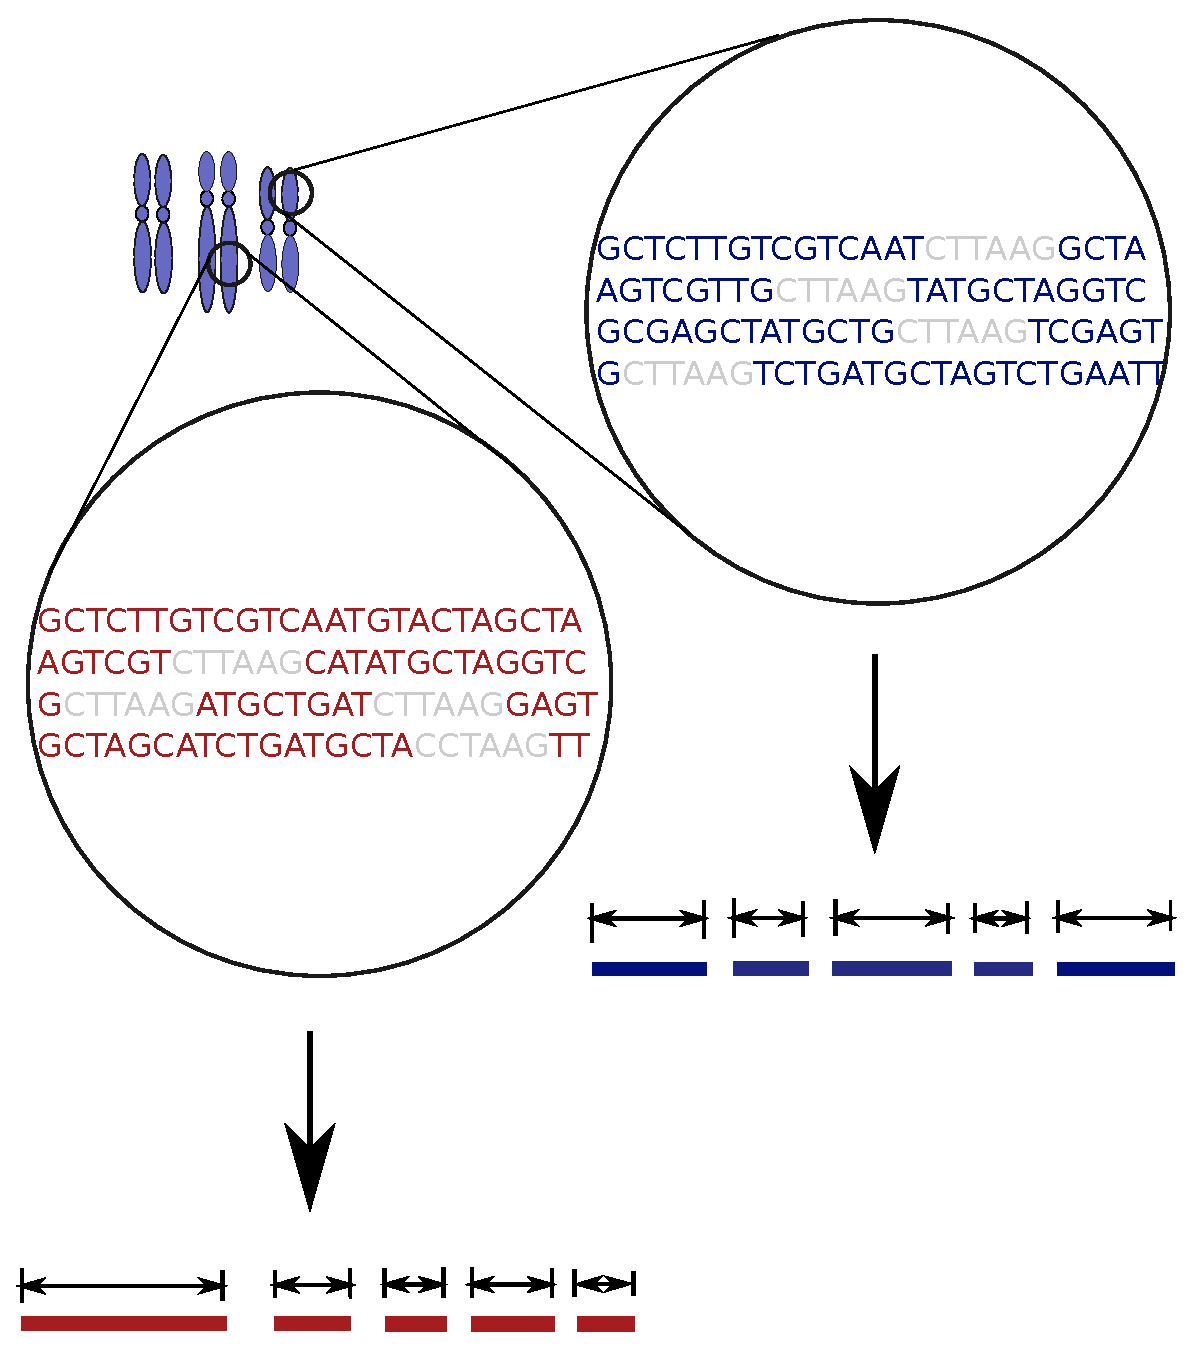
\includegraphics[width=0.35\textwidth]{../content/ormpub.eps}
   \label{figure:fig1}
 \end{SCfigure}


%%%%%%%%%%%%%%%%%%%%%%%%%%%%%%%%%%%%%%%%%%%%%%%%%%%%%%%%%%%%%%%%%%%%%%%%%%%%%%%%%%%%
% Paragraph 5: Previous related work,  including describing where SA and FM-index has been used in bioinformatics.

\paragraph{Our Contribution.}
We present the first index-based method for aligning contigs to an optical map.  
We call our tool $\twin$ to illustrate the association between the assembly and optical map as two representations of the genome sequence.  The first step of our procedure is to {\em in silico} digest the contigs with the set of restriction enzymes, computationally mimicking how each restriction enzyme would cleave the short segment of DNA defined by the contig.  Thus, {\em in silico digested contigs} are miniature optical maps that can be aligned to the much longer (sometimes genome-wide) optical maps.  The objective is to search and align the {\em in silico} digested contigs to the correct location in the optical map. 
By using a suitably-constructed FM-Index data structure~\cite{fm2005} built on the optical map,  we show that alignments between contigs and optical maps can be computed in time that is faster 
than competing methods by more than two orders of magnitude.  

%SOMA \cite{Nagarajan08} uses a dynamic programming algorithm to find optimal alignments under a formulation that allows for missed or spurious restriction sites in either sequence.   BACop \cite{Zhou09} also uses a dynamic programming algorithm and uses a scoring scheme that gives more weight to contigs with higher fragment density. AGORA \cite{AGORA} use a greedy exact matching strategy on simulated data.  Gentig \cite{Anantharaman01} and software developed by Valouev \textit{et al.} \cite{Valouev06} both use dynamic programming to address the closely related task of finding alignments between optical maps.

$\twin$ takes as input a set of contigs and an optical map, and produces a set of alignments.  The alignments are output in Pattern Space Layout (PSL) format, allowing them to be visualized using any PSL visualization software, such as IGV~\cite{igv}.  $\twin$ is specifically designed to work on a wide range of genomes, anything from relatively small genomes, to large eukaryote genomes.  Thus, we demonstrate the effectiveness of $\twin$ on {\em Yersinia kristensenii}, rice, and budgerigar genomes.  Rice and budgerigar have genomes of total sizes 430 Mb and 1.2 Gb, respectively. {\em Yersinia kristensenii}, a bacteria with genome size of 4.6 Mb, is the smallest genome we considered.   Short read sequence data was assembled for these genomes, and the resulting contigs were aligned to the respective optical map.   We compared the performance of our tool with available competing methods; specifically, the method of Valouev et al.~\cite{Valouev06} and SOMA~\cite{Nagarajan08}.  $\twin$ has superior performance on all datasets, and is demonstrated to be the only current method that is capable of completing the alignment for the budgerigar genome in a reasonable amount of CPU time; SOMA~\cite{Nagarajan08} required over 77 days of machine time to solve this problem, whereas, $\twin$ required just 35 minutes. Lastly, we verify our approach on simulated {\em E. coli} data by showing our alignment method found correct placements for the {\em in silico} digested contigs on a simulated optical map.     $\twin$ is available for download at \url{http://www.cs.colostate.edu/twin}. 

\paragraph{Roadmap.}
We review related tools for the problem in the remainder of this section. Section~\ref{sec-background} 
then sets notation and formally lays the data structural tools we make use of. 
Section~\ref{sec-methods} gives details of our approach. We report our experimental results in 
Section~\ref{sec-results}. Finally, Section~\ref{sec-discussion} offers reflections and some potentially 
fruitful avenues future work may take.

\paragraph{Related Work.}
The most recent tools to make use of optical mapping data in the context of assembly are AGORA~\cite{agora} and SOMA~\cite{Nagarajan08}. AGORA~\cite{agora} uses the optical map information to constrain de Bruijn graph construction with the aim of improving the resulting assembly. SOMA~\cite{Nagarajan08} is a scaffolding method that uses an optical map and is specifically designed for short-read assemblies. SOMA requires an alignment method for scaffolding and implements an $O(n^2 m^2)$-time dynamic programming algorithm. Gentig~\cite{Anantharaman01}, and software developed by Valouev et al.~\cite{Valouev06} also use dynamic programming to address the closely related task of finding alignments between optical maps. Gentig is not available for download.  BACop~\cite{Zhou09} also uses a dynamic programming algorithm and corresponding scoring scheme that gives more weight to contigs with higher fragment density. Antoniotti et al.~\cite{antoniotti} consider the unique problem of validating an optical map by using assembled contigs. This method assumes the contigs are error-free. Optical mapping data was produced for Assemblathon 2~\cite{bradnam2013assemblathon}.














